\sys is a prototype of a distributed battery-free audio assistant agent. \sys is envisioned to be embedded in, for example, wallpapers and furniture coverage to turn these objects to smart and controllable ones. The distributed nature of the \sys system enables it to exploit the inherent randomness of intermittent devices to offer a reliable interaction. 

\sys is a battery-less distributed microphone. It operates intermittently, when a threshold amount of energy accumulates.  

Audio is recorded for a fixed time period. After that, if the audio recording has finished successfully, the recording is divided into smaller parts called \textit{frames} and speech recognition is performed using an algorithm consisting of three steps:
\begin{enumerate*}
	\item endpoint detection
	\item feature extraction
	\item feature matching
\end{enumerate*}.
This steps are also depicted in figure \ref{fig:mic}.

\begin{figure}
	\centering
	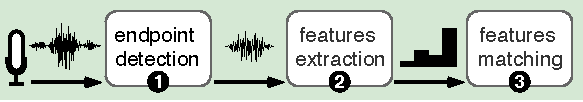
\includegraphics[width=\columnwidth]{figures/distributedMicrophone}
	\caption{ (1) endpoint detection algorithms extract the part of the signal corresponds to the input word, (2) feature extraction calculates the energy spectrum of the trimmed signal, and (3) feature matching searches the local database for the closest word}
	\label{fig:mic}
\end{figure}

%\textit{Endpoint detection} determines if there is a word in the recorded audio sample and, if there indeed is, the location of the word inside the recording is determined. There are several methods for doing endpoint detection. Two of them have been implemented and tested: power based and zero crossing rate (ZCR) based. The power based method estimates the energy of the audio signal by calculating the sum of amplitudes squared ($E = \sum A^2$) for each frame. The ZCR method counts how often the zero line is crossed per frame. The zero line in this case is equal to the microphone offset.

During \textit{feature extraction} on frames containing the word Fast Fourier Transform is applied to obtain the energy spectrum. 
The energy spectrum is then sorted into a feature vector, where each vector value holds the total energy of a specific frequency range. Finally each vector value is normalized over the total vector energy.

After that, \textit{feature matching} is performed, where the features of the recorded word are compared against a local database to find the most similar word in the database.
There exist many feature matching methods, yet only few are able to run under the constraints of an intermittent system.
Two methods have been implemented and tested. The first is Dynamic Time Warping (DTW), which is able to compare two sequences of data, even when they vary in speed. This way if a word is spoken slower or faster, the algorithm can compensate for that.
The second is a method that linearly compares two feature vectors. This requires less computations than DTW.

\subsection{Hardware description}
we used MSP430RF5994~\cite{} an ultra-low-power microcontroller to drive the PMM-3738-VM1010-R microphone that features zero power listening and wake-on-sound technology~\cite{}. A BQ25570EVM-206 solar power harvester connected to a pair of SLMD121H04L solar panels intermittently powers a \sys sensor. For some experiments simulated intermittent power is used. For debugging, we used saleae logic analyzer~\cite{}. 

\subsection{Implementation}
During recording a sample rate was used of 7812 Hz, which covers the human voice frequency range. The used frame size was 256 samples. This size was beneficial for doing a Fast Fourier Transform and corresponds to approximately 33 milliseconds of speech.

For normalization an integer log function was applied on every value, divided by the average log.
The whole algorithm is implemented using only integer / fixed point arithmetic.

%DTW is a well known method in speech recognition.
In the linear comparing method the feature vectors of two words are compared successively, not accounting for differences in the speed of pronunciation. If two words vary in length, the last frames cannot always be compared and instead a penalty is applied linear to the length difference.

In between the different steps (see figure \ref{fig:mic}) checkpoints in non-volatile memory are used to assure progress while running on intermittent power. In some cases additional checkpoint were used inside the steps.

